\documentclass[letterpaper]{article}

%----------------------------------------------------------------------
% Packages

\usepackage{amsmath}
\usepackage{amsfonts}
\usepackage{amssymb}
\usepackage{mathtools}
\usepackage{cancel}
\usepackage{graphicx}
\usepackage{xcolor}
\usepackage{tikz, tcolorbox}
\usepackage{siunitx}
\usepackage{geometry}
\usepackage{fancyhdr}
\usepackage{lastpage}
\usepackage{placeins}


%----------------------------------------------------------------------
% Custom Math Commands

% General Shortcuts
\newcommand{\defeq}{\vcentcolon=}  % Define as
\newcommand{\R}{\mathbb{R}}        % Real Numbers
\newcommand{\C}{\mathbb{C}}        % Complex Numbers
\newcommand{\N}{\mathbb{N}}        % Natural Numbers (0, 1, 2, ...)
\newcommand{\Z}{\mathbb{Z}}        % Integers (..., -2, -1, 0, 1, 2, ...)
\newcommand{\Q}{\mathbb{Q}}        % Rational Numbers

% Linear Algebra Shortcuts
\newcommand{\bv}[1]{\boldsymbol{#1}}      % bold vector quantity
\newcommand{\norm}[1]{|| {#1} ||_1}       % generic norm
\newcommand{\onenorm}[1]{|| {#1} ||_1}    % one norm
\newcommand{\twonorm}[1]{|| {#1} ||_2}    % two norm
\newcommand{\infnorm}[1]{|| {#1} ||_\inf} % infinty norm

% Probability and Statistics Shortcuts
\newcommand{\E}[1]{\textrm{E}\left[#1\right]}
\newcommand{\Var}[1]{\textrm{Var}\left(#1\right)}
\newcommand{\Cov}[1]{\textrm{Cov}\left(#1\right)}

% Navigation Shortcuts
\newcommand{\navvec}[3]{\boldsymbol{#1}^{\,#2}_{#3}}              % navigation vector
\newcommand{\navmeas}[3]{\tilde{\boldsymbol{#1}}^{\,#2}_{#3}}     % navigation measurement
\newcommand{\navest}[3]{\hat{\boldsymbol{#1}}^{\,#2}_{#3}}        % navigation estimate
\newcommand{\navC}[2]{C^{\,#1}_{#2}}                              % coordinate frame transformation
\newcommand{\quat}[2]{q^{#1}_{#2}}                                % quaternion

% Misc.
\newcommand{\MATLAB}{MATLAB\,\textsuperscript{\tiny\textregistered}\,}


%----------------------------------------------------------------------
% Begin Document

\begin{document}
	
	
	%------------------------------------------------------------------
	% Title
	
	\title{Inverse Problems for Inertial Sensor Calibration}
	\author{David L. Olson}
	\date{\today}
	
	\maketitle
	
	%------------------------------------------------------------------
	% Table of Contents
	
	\tableofcontents
	
	%------------------------------------------------------------------
	% Abstract
	
	\newpage
	\begin{abstract}
	
	Inertial sensors are vital to navigation, guidance, and control (NGC) for a variety of vehicles. Inertial sensors such as accelerometers and gyroscopes measure specific and angular velocity respectively which are mechanized to produce a position, velocity, and attitude (PVA) solution \cite{groves2013principles}. All inertial sensors are subject to deterministic and stochastic error which require careful calibration and characterization before utilizing inertial sensors in a vehicle application. In industry, the current state of the art for inertial sensor calibration has made little advancement over the past couple decades, where calibration data is collected and post-processed using basic statistics to compute basic error model parameters. In the past, improved fidelity for calibration required purchasing higher and higher precision equipment, which eventually succumbs to the law of diminishing returns.
	
	However, ongoing research addressing inertial sensor calibration seeks to break dependence on high-cost high-precision test equipment by introducing advanced estimation techniques and stochastic filtering to maintain high fidelity calibration performance \cite{ImprovedIMUCalibrationProcedures,Rahimi763,8943630,9851744,aCalibrationMethodForSixAccelerometerINS}. While various papers only tackle small pieces of an entire calibration procedure, there is an opportunity to cast inertial sensor calibration as an inverse problem to provide a holistic methodology to the field. The forward problem is simply the process of transforming true dynamic inputs acting on the sensor to sensor outputs which is subject to error. Then, the inverse problem takes the form of calibration in which calibration parameters are estimated from collected sensor data. Using inverse problem techniques, calibration parameter estimation can advance beyond basic statistical techniques for higher fidelity performance to include covariance propagation to assign confidence to final calibration parameters. In addition, estimation may be performed in real-time during the collection of calibration data, alleviating logistical and programmatic troubles for an inertial test laboratory.
	
	The author plans to build upon previous work \cite{GeneralizedFramework} which homogenized multiple IEEE standards for varying accelerometer and gyroscope technologies \cite{IEEE_std_1293-2018,IEEE_std_1431-2004,IEEE_std_952-2020,IEEE_std_292-1969,IEEE_std_517-1974,IEEE_std_647-2006,IEEE_std_813-1988} which provide highly detailed inertial sensor error models. Inertial sensor data will be simulated using \cite{RTSim} which can provide true inertial sensor measurements which can then be corrupted with error and noise. Then, inverse problem techniques may be demonstrated and contrasted with traditional methods to showcase improvements and possible limitations to using these new highly detailed models. Higher fidelity calibration yields increased sensor accuracy, which ultimately enhances inertial navigation capabilities for a wide range of vehicle applications. 
	
\end{abstract}
	
	
	%------------------------------------------------------------------
	% Header and Footer
	
	\thispagestyle{empty}
	\pagestyle{empty}
	
	\fancyhead{}
	\fancyfoot{}
	
	\thispagestyle{fancy}
	\pagestyle{fancy}
	
	\fancyhead[L]{\textbf{Inverse Problems}}
	\fancyhead[R]{\textbf{David L. Olson}}
	
	\fancyfoot[L]{\textbf{Term Project}}
	\fancyfoot[R]{\thepage\ of \pageref{LastPage}}
	
	
	%------------------------------------------------------------------
	% Begin Technical Content
	
	\newpage
	%----------------------------------------------------------------------
% Introduction

\begingroup
\allowdisplaybreaks

\section{Introduction}

A key challenge for self-driving cars is solving the navigation problem which requires determining the position, velocity, and attitude (PVA) of the vehicle. Navigation is an interdisciplinary field of engineering which seeks to fuse measurements of many different sensors such as inertial measurement units (IMUs), global positioning system (GPS) receivers, and a large variety of other sensors to form a PVA solution. It is crucial to not only formulate a navigation solution but also to track the uncertainty of that solution, which can play an important role in decision-making and risk-assessment for autonomous self-driving vehicle applications.

IMUs contain accelerometers and gyroscopes generally in all three Cartesian axes which measure specific force and angular velocity respectively. These measurements are integrated to provide a PVA solution, but an IMU-only solution will drift away from truth unbounded due to the integration of sensor noise and other errors. An inertial navigation system (INS) integrates the IMU measurements and then uses GPS to provide accurate measurements of position to fuse with the IMU solution typically via a Kalman filter thus combating any position error drift. This allows for long-term accurate navigation suitable for a self-driving car traveling across the country.

One particular challenge for navigation regarding self-driving cars is forming back-up modes of navigation when GPS signals are temporarily unavailable. This is especially important in urban environments where tall buildings and tunnels can cause signal blockages. Lack of GPS signals are problematic for an INS as its performance is dependent on receiving those signals, and the IMU-only solutions will drift away quickly from ground truth. Inertial-only navigation is suitable for short periods such as temporary GPS signal blockages, but the duration of a suitable inertial-only navigation is highly dependent on the quality of sensors contained within an IMU. This dilemma, among any others, motivates the need for rigorous IMU calibration and compensation.


\subsection{IMU Calibration and Compensation as a Forward/Inverse Problem}

Accelerometers and gyroscopes are subject to a variety of error sources such as biases, scale factor imperfections, axis misalignments, noise, and many others. IMU calibration is the process of characterizing these error sources, while compensation is the process of correcting measurements in real-time to provide the most accurate and precise measurements possible. The better these error sources are characterized, the slower that the IMU-only navigation solution will drift away from truth. 

Inertial sensor calibration can be treated as an inverse problem. Consider an accelerometer as an example where the ideal forward model is quite straight forward; specific force in equals specific force out. Unfortunately in practice, we are not quite so lucky. Any error in the forward model is defined as

\begin{align*}
	\Delta f \defeq \tilde{f} - f
\end{align*}

where $\Delta f$ is the measurement error, $\tilde{f}$ is the specific force measured by the sensor which is subject to error, and $f$ is the true specific force acting on the accelerometer. The same applies to gyroscope measurements. 

\begin{align*}
	\Delta \omega \defeq \tilde{\omega} - \omega
\end{align*}

Inertial sensor errors $\Delta f$ and $\Delta \omega$ are subject to both deterministic and stochastic error and any number of contributing factors can make up these terms.

Now consider an IMU which contains three accelerometers and three gyroscopes arranged to point in a standard Cartesian right-handed coordinate frame. A basic framework


	
	\newpage
	%----------------------------------------------------------------------
% Methods

\begingroup
\allowdisplaybreaks

\section{Methods}

 Consider an IMU under test strapped down to a three axis rotational test bed. The rotational test bed provides measurements of angular position and angular rate along each test axis. As exemplar hardware, the unit under test will be a STIM 300 IMU from Safran and the 210C Series Three Axis Position and Rate Table System from Ideal Aerosmith.


\subsection{STIM 300 IMU Specifications} \label{sec: stim 300 imu specifications}
 
The STIM 300 IMU, henceforth referred to as the unit under test (UUT), provides measurements of specific force and angular velocity. While the true forward model is unknown, it will be assumed that the basic forward model in equation \ref{eq: compact IMU forward error model} will sufficiently model the error of the device. Assuming the UUT uses the "10g" variant of accelerometers, bounds for the accelerometer-related model parameters are provided in table 5-5 of the specification sheet \cite{stim300SpecSheet}.
 
\begin{itemize}
	\item Bias: $|b_a| \leq 7.5 \times 10^{-3} g$
	\item Scale Factor Error : $|s_a| \leq 200 \,\textrm{ppm}$
	\item Misalignment: $|m_a| \leq 1\times 10^{-3} \,\textrm{rad}$ 
\end{itemize}
 
The accelerometers are also subject to zero-mean Gaussian noise with a velocity random walk (VRW) value of $0.07 \unit{\meter\per\second\per\sqrt\hertz}$, which translates to a $\sigma_a = \frac{0.07}{60} = 0.0012 \unit{\meter\per\second}$. Likewise, \cite{stim300SpecSheet} provides bounds for the gyroscopes in table 5-3. 
 
\begin{itemize}
	\item Bias: $|b_g| \leq 250 \unit{\degree\per\hour}$
	\item Scale Factor Error : $|s_g| \leq 500 \,\textrm{ppm}$
	\item Misalignment: $|m_g| \leq 1\times 10^{-3} \,\textrm{rad}$ 
\end{itemize}
 
The gyroscopes are also subject to zero-mean Gaussian noise with an angle random walk (ARW) value of $0.15 \unit{\degree\per\sqrt\hour}$ which translates to a $\sigma_g = \frac{0.15}{60}\frac{\pi}{180} = 4.3633 \times 10^{-5} \unit{\radian\per\second}$.

For simulation purposes, true model parameters will be selected within these bounds.


%\subsection{2013C Series Position and Rate Table System Specifications}
%
%The 2013C Series Position and Rate Table System, henceforth referred to as the test bed, is able to spin and point the UUT in all directions within Cartesian space. Per the specification sheet \cite{threeAxisRateTableTable}, each axis can spin with an accuracy of $\pm 0.001\%$ and point with an accuracy $\pm 15 \unit{\arcsecond}$.
%
%For simplicity, let measurements of angular position and angular rate be subject to zero-mean Gaussian noise with the inaccuracies above interpreted as the 3-sigma bound. For additionally simplicity, assume that each Euler angle representing the attitude of the UUT is subject to the root mean square of the test bed's pointing accuracy.
%
%\begin{align*}
%	\sigma_\theta \approx \sqrt{\frac{1}{3} 15 \unit{\arcsecond} + \frac{1}{3} 15 \unit{\arcsecond} + \frac{1}{3} 15 \unit{\arcsecond}} = 8.5 \times 10^{-3} \,\unit{\radian}
%\end{align*}
%
%Likewise, assume that the resulting angular velocity measurements of the UUT derived from the test bed are the root mean square of the test bed's spinning accuracy when spinning at $100 \unit{\degree\per\sec}$.
%
%\begin{align*}
%	\sigma_\omega \approx \frac{\pi}{180} \sqrt{\frac{1}{3} 0.1 + \frac{1}{3} 0.1 + \frac{1}{3} 0.1} = 9.6 \times 10^{-3} \,\unit{\radian\per\second}
%\end{align*}
%
%The approximations are very crude, however expressing their uncertainty as a Normal distribution allows for a consistent application in the methods ahead.


\subsection{Simulating Calibration Data and Model Parameters}

Rotational motion on the test bed will be simulated by developing a true sequence of angular velocities $\bv{\omega}$ across time $t$ experienced by the UUT. The attitude of the UUT, represented by the direction cosine matrix $C\left(t\right)$, will be integrated in discrete steps such that the $k^{\textrm{th}}$ step in the sequence is 

\begin{align}
	C\left(t_k\right) = C_0 \prod_{i = 1}^k e^{\left[\bv{\omega}\left(t_i\right) \times\right] \Delta t}
\end{align}  

where $\left[\bv{\omega}\left(t_i\right) \times\right]$ is a skew-symmetric matrix and $\Delta t$ is the time step. While the test bed rotates, the accelerometers will each be measuring components of the normal force from the test bed resulting from the acceleration due to gravity $g$. For each time step $k$, the true specific force quantity is given below.

\begin{align}
	\bv{f}\left(t_k\right) = C\left(t_k\right) \begin{bmatrix} 0 \\ 0 \\ g \end{bmatrix}
\end{align}

In the simulation, it will be assumed that quantities $\bv{\omega}$ and $\bv{f}$ will be available through measurement outputs of the test bed itself. Measurements of these quantities from the UUT will be corrupted with measurement error according to equations \ref{eq: expanded IMU forward error model}. The values of the model parameters are recorded in table \ref{tab: UUT simulated model parameters} and are selected with reasonable orders of magnitude as discussed in section \ref{sec: stim 300 imu specifications}. 

\begin{table}[h!]
	\centering
	\begin{tabular}{|p{4cm}|p{3.5cm}|p{3.5cm}|}
		\hline
		\textbf{Model Parameter} & \textbf{Accel Values} & \textbf{Gyro Values} \\ \hline
		Fixed Bias X & $0.0628 \,\unit{\meter\per\second\squared}$ & $0.48481 \times 10^{-3} \,\unit{\radian\per\second}$ \\ \hline
		Fixed Bias Y & $-0.0510 \,\unit{\meter\per\second\squared}$ & $0.14544 \times 10^{-3}  \,\unit{\radian\per\second}$ \\ \hline
		Fixed Bias Z & $0.0363 \,\unit{\meter\per\second\squared}$ & $1.2120 \times 10^{-3}  \,\unit{\radian\per\second}$ \\ \hline
		Scale Factor Error X & $150 \,\textrm{ppm}$ & $450 \,\textrm{ppm}$ \\ \hline
		Scale Factor Error Y & $-175 \,\textrm{ppm}$ & $-300 \,\textrm{ppm}$ \\ \hline
		Scale Factor Error Z & $198 \,\textrm{ppm}$ & $175 \,\textrm{ppm}$ \\ \hline
		Misalignment XY & $0.1 \,\unit{\milli\radian}$ & $-0.1 \,\unit{\milli\radian}$ \\ \hline
		Misalignment XZ & $-0.2 \,\unit{\milli\radian}$ & $0.2 \,\unit{\milli\radian}$ \\ \hline
		Misalignment YX & $0.3 \,\unit{\milli\radian}$ & $-0.3 \,\unit{\milli\radian}$ \\ \hline
		Misalignment YZ & $-0.4 \,\unit{\milli\radian}$ & $0.4 \,\unit{\milli\radian}$ \\ \hline
		Misalignment ZX & $0.5 \,\unit{\milli\radian}$ & $-0.5 \,\unit{\milli\radian}$ \\ \hline
		Misalignment ZY & $-0.6 \,\unit{\milli\radian}$ & $0.6 \,\unit{\milli\radian}$ \\ \hline
	\end{tabular}
	\caption{UUT Simulated Model Parameters}
	\label{tab: UUT simulated model parameters}
\end{table}
\FloatBarrier

Capabilities for simulating calibration sequences on test beds and IMU error models have been developed in \MATLAB. 


\subsection{Formulating IMU Calibration as a Discrete Linear Inverse Problem}

Recall the system of equations from equation \ref{eq: expanded IMU forward error model} and consider the $x$-axis accelerometer measurements.

\begin{align*}
	\tilde{f}_x = \left(1 + s_{a,x}\right) f_x + m_{a,xy} f_y + m_{a,xz} f_z + b_{a,x}
\end{align*}

The equation above can be re-arranged to express the model parameters as a function of the accelerometer error $\Delta f = \tilde{f} - f$. 

\begin{align*}
	\tilde{f}_x &= \left(1 + s_{a,x}\right) f_x + m_{a,xy} f_y + m_{a,xz} f_z + b_{a,x} \\
	\\
	\tilde{f}_x - f_x &= b_{a,x} + s_{a,x} f_x + m_{a,xy} f_y + m_{a,xz} f_z \\
	\\
	\Delta f_x &= b_{a,x} + s_{a,x} f_x + m_{a,xy} f_y + m_{a,xz} f_z
\end{align*}

Assuming that both the UUT and test bed are able to provide synchronized measurements at the same sampling frequency, a series of measurements from these devices can be organized into another system of equations. 

\begin{align} \label{eq: expanded block of GM = d}
	\begin{bmatrix} 
		1 & f_x[1] & f_y[1] & f_z[1] \\ 1 & f_x[2] & f_y[2] & f_z[2] \\ \vdots & \vdots & \vdots & \vdots \\ 1 & f_x[m] & f_y[m] & f_z[m]
	\end{bmatrix} \begin{bmatrix}
		b_{a,x} \\ s_{a,x} \\ m_{a,xy} \\ m_{a,xz}
	\end{bmatrix} = \begin{bmatrix}
		\Delta f_x[1] \\ \Delta f_x[2] \\ \vdots \\ \Delta f_x[m]
	\end{bmatrix}
\end{align}

This system of equations can be expressed in the form $G\bv{m} = \bv{d}$. In this expression, "true" measurements $f_x[n],\,f_y[n],\,f_z[n]$ within the model operator are computed from measurements provided by the test bed, and the model parameters are various calibration factors from the forward model. Elements of the data vector $\bv{d}$ are the difference of the UUT output and test bed output such that $d[n] = \tilde{f}_x[n] - f_x[n]$.

Let $F$ be the model operator demonstrated by equation \ref{eq: expanded block of GM = d}.

\begin{align} \label{eq: F}
	F &\defeq \begin{bmatrix} 
		1 & f_x[1] & f_y[1] & f_z[1] \\ 1 & f_x[2] & f_y[2] & f_z[2] \\ \vdots & \vdots & \vdots & \vdots \\ 1 & f_x[m] & f_y[m] & f_z[m]
	\end{bmatrix},\,\,\, F \in \R^{m \times 4}
\end{align}

Then, the discrete linear inverse problem for all accelerometer calibration parameters given in equation \ref{eq: expanded IMU forward error model} can defined below.

\begin{align} \label{eq: Gm = d for all accel parameters}
	G_a \bv{m}_a &= \bv{d}_a \notag\\
	\\
	\begin{bmatrix} 
		F & 0_{m \times 4} & 0_{m \times 4} \\
		0_{m \times 4} & F & 0_{m \times 4} \\
		0_{m \times 4} & 0_{m \times 4} & F \\
	\end{bmatrix} \begin{bmatrix}
		b_{a,x} \\ s_{a,x} \\ m_{a,xy} \\ m_{a,xz} \\ b_{a,y} \\ m_{a,yz} \\ s_{a,y} \\ m_{a,yz} \\ b_{a,z} \\ m_{a,zx} \\ m_{a,zy} \\ s_{a,z}
	\end{bmatrix} &= \begin{bmatrix}
		\Delta f_x[1] \\ \vdots \\ \Delta f_x[m] \\ \\ \Delta f_y[1] \\ \vdots \\ \Delta f_y[m] \\ \\ \Delta f_z[1] \\ \vdots \\ \Delta f_z[m]
	\end{bmatrix} \notag
\end{align}

Likewise, let $\Omega$ be the model operator for all gyroscope measurements specific to one sensor. 

\begin{align} \label{eq: Omega}
	\Omega &\defeq \begin{bmatrix} 
		1 & \omega_x[1] & \omega_y[1] & \omega_z[1] \\ 1 & \omega_x[2] & \omega_y[2] & \omega_z[2] \\ \vdots & \vdots & \vdots & \vdots \\ 1 & \omega_x[m] & \omega_y[m] & \omega_z[m]
	\end{bmatrix},\,\,\, \Omega \in \R^{m \times 4}
\end{align}

Then, the discrete linear inverse problem for all gyroscope calibration parameters given in equation \ref{eq: expanded IMU forward error model} can defined below.

\begin{align} \label{eq: Gm = d for all gyro parameters}
	G_g \bv{m}_g &= \bv{d}_g \notag\\
	\\
	\begin{bmatrix} 
		\Omega & 0_{m \times 4} & 0_{m \times 4} \\
		0_{m \times 4} & \Omega & 0_{m \times 4} \\
		0_{m \times 4} & 0_{m \times 4} & \Omega \\
	\end{bmatrix} \begin{bmatrix}
		b_{g,x} \\ s_{g,x} \\ m_{g,xy} \\ m_{g,xz} \\ b_{g,y} \\ m_{g,yz} \\ s_{g,y} \\ m_{g,yz} \\ b_{g,z} \\ m_{g,zx} \\ m_{g,zy} \\ s_{g,z}
	\end{bmatrix} &= \begin{bmatrix}
		\Delta \omega_x[1] \\ \vdots \\ \Delta \omega_x[m] \\ \\ \Delta \omega_y[1] \\ \vdots \\ \Delta \omega_y[m] \\ \\ \Delta \omega_z[1] \\ \vdots \\ \Delta \omega_z[m]
	\end{bmatrix} \notag
\end{align}


\subsection{Assessing Singular Values}

Prior to solving the inverse problem, we must ensure that the problem is not ill-conditioned. This is accomplished by performing a singular value decomposition (SVD) on the model operators $\Omega$ and $F$ respectively from equations \ref{eq: Omega} and \ref{eq: F}. Although these model operators may appear to be full-rank when calling \MATLAB's \verb|rank()| function, some singular values may be poorly scaled. Therefore, it is essential to verify that the singular values are suitable for each new motion profile run on the three-axis rate table. 

If the singular values are poorly scaled, it may be necessary to compute a truncated SVD solution or regularize the solution. In both cases, this takes away the opportunity to assess the resulting covariances and correlations between model parameters as the model null-space is now non-trivial and may lead to a biases solution in the model parameters. 


\subsection{L2 Regression without a Known Normal Distribution} \label{sec: L2 regresssion}

Although a typical IMU specification sheet contains values of VRW and ARW which relate to the white noise present on each sensor channel, in practice each individual sensor is subject to its own amount of white noise. Therefore, to be consistent with application, we will assume that each sample is dependent and identically distributed, although the standard deviation associated with the white noise will be unknown. Therefore, casting this problem as a weighted least squares problem is not feasible. Additionally in practice, it is not a safe assumption to assume that the power of the white noise signal is equally distributed at all frequencies, introducing noise color, however this will be ignored for both simulation and evaluation purposes. 

Since the inverse problem can not be casted as a weighted least squares problem, the inverse problem will be solved via the normal equations (assuming the model operator is not ill-conditioned) without any scaling applied to the model operators. 

\begin{align} \label{eq: L2 Regression}
	\bv{m}_{a,L2} &= \left(G_a^T G_a\right)^{-1} G_a^T \bv{d_a} \notag\\
	\\
	\bv{m}_{g,L2} &= \left(G_g^T G_g\right)^{-1} G_g^T \bv{d_g} \notag
\end{align}

Without a known standard deviation, we instead must estimate the resulting standard deviation from the residuals after performing the least squares fit. 

\begin{align} \label{eq: estimated sigma}
	s_a = \frac{\twonorm{G_a \bv{m}_{a,L2} - \bv{d}_a}}{\sqrt{m - n}} \notag\\
	\\
	s_g = \frac{\twonorm{G_g \bv{m}_{g,L2} - \bv{d}_g}}{\sqrt{m - n}} \notag
\end{align}

With these estimated standard deviations, we can approximate the model covariance. 

\begin{align} \label{eq: estimated model covaraince}
	\tilde{C}_a = s_a^2 \left(G_a^T G_a\right)^{-1} \notag\\
	\\
	\tilde{C}_g = s_g^2 \left(G_g^T G_g\right)^{-1} \notag
\end{align}

Rather than using a Normal distribution to determine the 95\% confidence interval, we must use the Student's $t$ distribution instead. In this use case, the degree of freedom with be very large which should well-approximate the normal distribution. 

\begin{align} \label{eq: confidence intervals}
	m_{a,L2_i} &\pm t_{0.95,\nu} \sqrt{\tilde{C}_{a_{i,i}}}  \notag\\
	\\
	m_{g,L2_i} &\pm t_{0.95,\nu} \sqrt{\tilde{C}_{g_{i,i}}}  \notag
\end{align}

In addition to the model covariance, the correlation between each model parameter will also be examined. 


\subsection{Motion Profile Evaluation}

First, we will investigate using traditional calibration data to solve the inverse problem and make comparisons to the traditional post-processing methods for IMU calibration. 

Then, we will investigate three unique motion profiles for evaluation.

\begin{enumerate}
	\item \textbf{Single-Axis Tilts in One Direction}
	\item \textbf{Single-Axis Tilts in Two Directions}
	\item \textbf{Multi-Axis Tilts in All Directions}
\end{enumerate}
	

The dynamics of each motion profile will cause varying model fits, covariances, and correlations. These insights will be useful to those needing to develop new motion profiles to calibrate IMUs. Their Euler angle profiles are proved in figures \ref{fig: MP1 Euler Angle Profile}, \ref{fig: MP2 Euler Angle Profile}, and \ref{fig: MP3 Euler Angle Profile}.

\begin{figure}[h] 
	\centering
	\includegraphics[width=0.5\textwidth]{./images/MP1_euler_angle_profile.eps}
	\caption{Motion Profile 1: Euler Angle Profile}
	\label{fig: MP1 Euler Angle Profile}
\end{figure}
\FloatBarrier

\begin{figure}[h] 
	\centering
	\includegraphics[width=0.5\textwidth]{./images/MP2_euler_angle_profile.eps}
	\caption{Motion Profile 2: Euler Angle Profile}
	\label{fig: MP2 Euler Angle Profile}
\end{figure}
\FloatBarrier

\begin{figure}[h] 
	\centering
	\includegraphics[width=0.5\textwidth]{./images/MP3_euler_angle_profile.eps}
	\caption{Motion Profile 3: Euler Angle Profile}
	\label{fig: MP3 Euler Angle Profile}
\end{figure}
\FloatBarrier

Then, we will analyze a motion profile designed to purposely be ill-conditioned to determine what model fit, if any, could be obtained if forced into this situation. This motion profile is provided in figure \ref{fig: MP4 Euler Angle Profile}.

\begin{figure}[h] 
	\centering
	\includegraphics[width=0.5\textwidth]{./images/MP4_euler_angle_profile.eps}
	\caption{Motion Profile 3: Euler Angle Profile}
	\label{fig: MP4 Euler Angle Profile}
\end{figure}
\FloatBarrier


	
	\newpage
	%----------------------------------------------------------------------
% Results

\begingroup
\allowdisplaybreaks

\section{Results}

\subsection{Traditional Calibration Sequence}

A traditional calibration sequence was simulated for a UUT with an assumed sample rate of $100 \,\unit{\hertz}$. Each test specified in table \ref{tab: traditional_calibration_tests} for a duration of $10 \,\unit{\second}$. All of the accelerometer test data were appended together to build the model operator $G_a$, and as well as all of the gyroscope test data to build $G_g$. Before proceeding with solving for the weighted least squares solution, a quick check was performed to ensure the both $G_a$ and $G_g$ were full rank. 

\begin{align}
	\textrm{rank}\left(G_a\right) &= 6,\,\,\, G_a \in \R^{60006 \times 12} \notag\\
	\\
	\textrm{rank}\left(G_g\right) &= 6,\,\,\, G_g \in \R^{60006 \times 12} \notag
\end{align}

The fact that both $G_a$ and $G_g$ are not full rank was not initially expected. However, given that the number of observations $m = 60006$ actually has many repeated rows as the UUT itself undergoes no changes in specific force and angular rate, this should not have been as much of a surprise. Instead of proceeding with solving for a solution, another calibration sequence was designed.







%******************************************************
% Single-Axis Motion
%******************************************************

\subsection{Single-Axis Motion Calibration Sequence}

In response to the lack of full rank in the previous experiment design, a new calibration sequence was designed to put axis of the UUT in motion in hopes of establishing model operators of full rank. Figures \ref{fig: single-axis angular velocity profile} and \ref{fig: single-axis euler angle profile} show the designed motion profile.

\begin{figure}[h] 
	\centering
	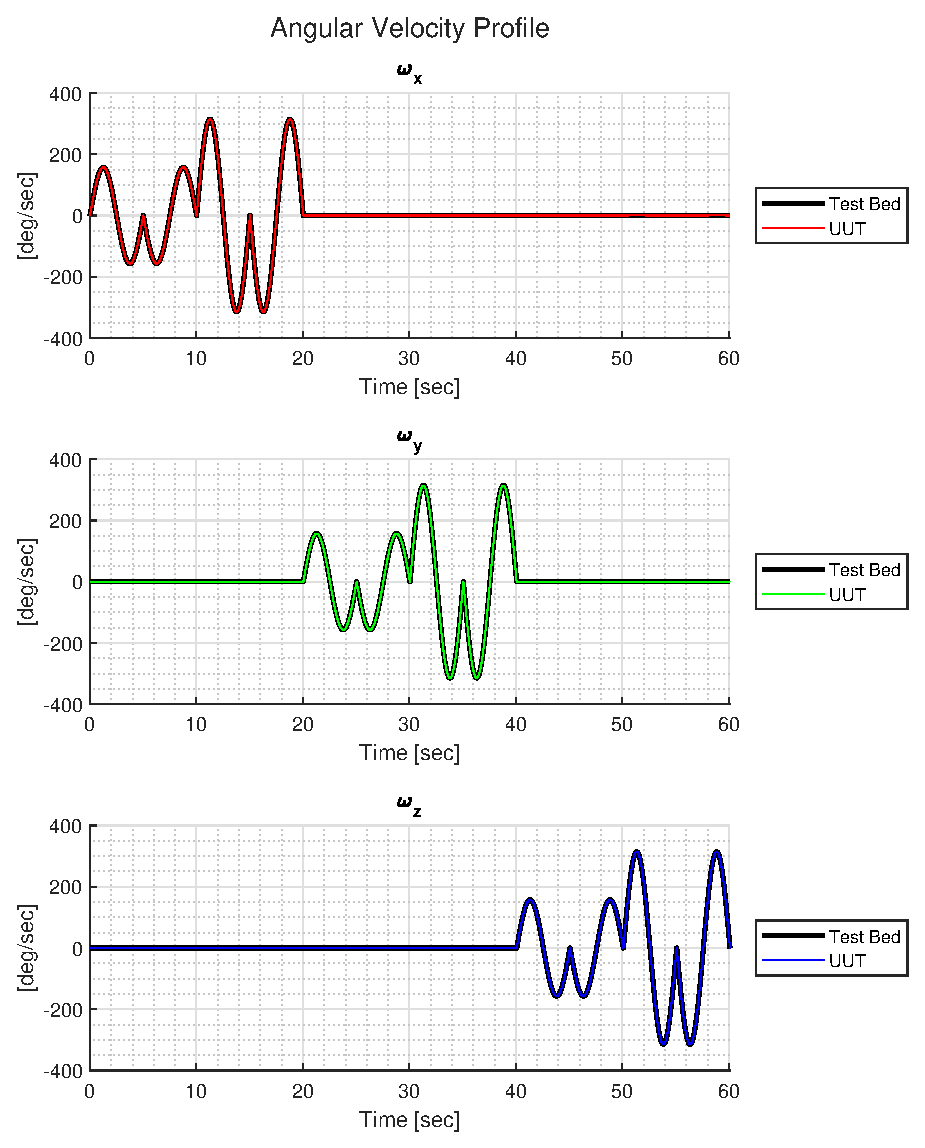
\includegraphics[width=0.65\textwidth]{./images/SAM_angular_velocity_profile.eps}
	\caption{Single-Axis Angular Velocity Profile}
	\label{fig: single-axis angular velocity profile}
\end{figure}
\FloatBarrier

\begin{figure}[h] 
	\centering
	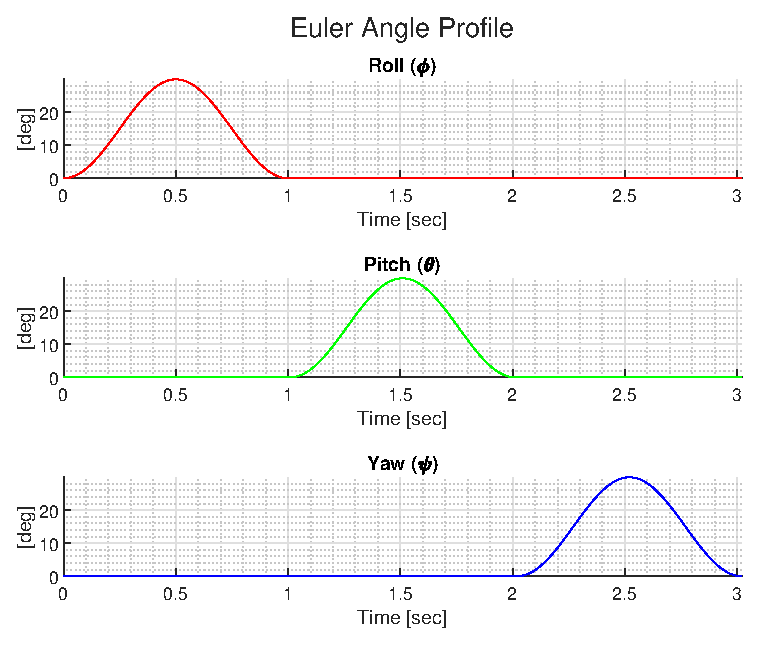
\includegraphics[width=0.65\textwidth]{./images/SAM_euler_angle_profile.eps}
	\caption{Single-Axis Euler Angle Profile}
	\label{fig: single-axis euler angle profile}
\end{figure}
\FloatBarrier

Due to the rotations of the test bed, the specific force is also altered as shown in figure \ref{fig: single-axis specific force profile}.

\begin{figure}[h] 
	\centering
	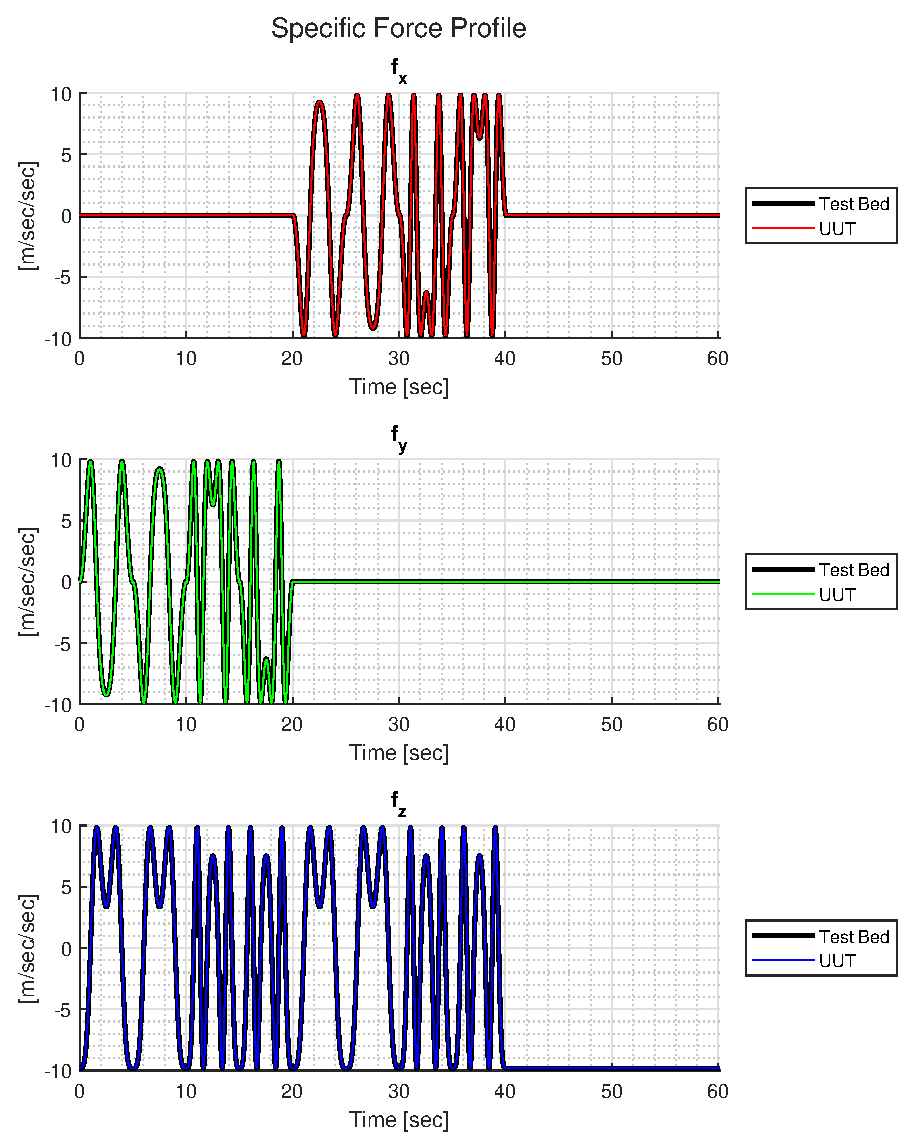
\includegraphics[width=0.65\textwidth]{./images/SAM_specific_force_profile.eps}
	\caption{Single-Axis Specific Force Profile}
	\label{fig: single-axis specific force profile}
\end{figure}
\FloatBarrier

\subsubsection{Model Operator Rank}

Even with new motion profiles, both model operators $G_a$ and $G_g$ are not full rank. 

\begin{align}
	\textrm{rank}\left(G_a\right) &= 12,\,\,\, G_a \in \R^{909 \times 12} \notag\\
	\\
	\textrm{rank}\left(G_g\right) &= 12,\,\,\, G_g \in \R^{909 \times 12} \notag
\end{align}

In response, a model solution was still obtained using the generalized inverse. This rank-deficiency is of the type "$p = n$ and $p < m$, in which the data null space is non-trivial but the model null space is trivial. This implies that the solution will be unique, but cannot fit the general data exactly. For both $G_a$ and $G_g$, a singular value decomposition (SVD) was performed and each decomposed matrix was truncated to the rank of the matrix. The generalized inverse model was formed accordingly below.

\begin{align}
	\bv{m}_{\dagger}^{a} &= V_{a,p} S_{a,p}^{-1} U_{a,p}^T \bv{d}_a \notag\\
	\\
	\bv{m}_{\dagger}^{g} &= V_{g,p} S_{g,p}^{-1} U_{g,p}^T \bv{d}_g \notag
\end{align}

Each model resolution matrix $R_m = V_p V_p^T$ shows that each model parameter has perfect resolution. The singular values for each model operator are shown in figures \ref{fig: single-axis accelerometer singular values} and \ref{fig: single-axis gyroscope singular values}. 

\begin{figure}[h] 
	\centering
	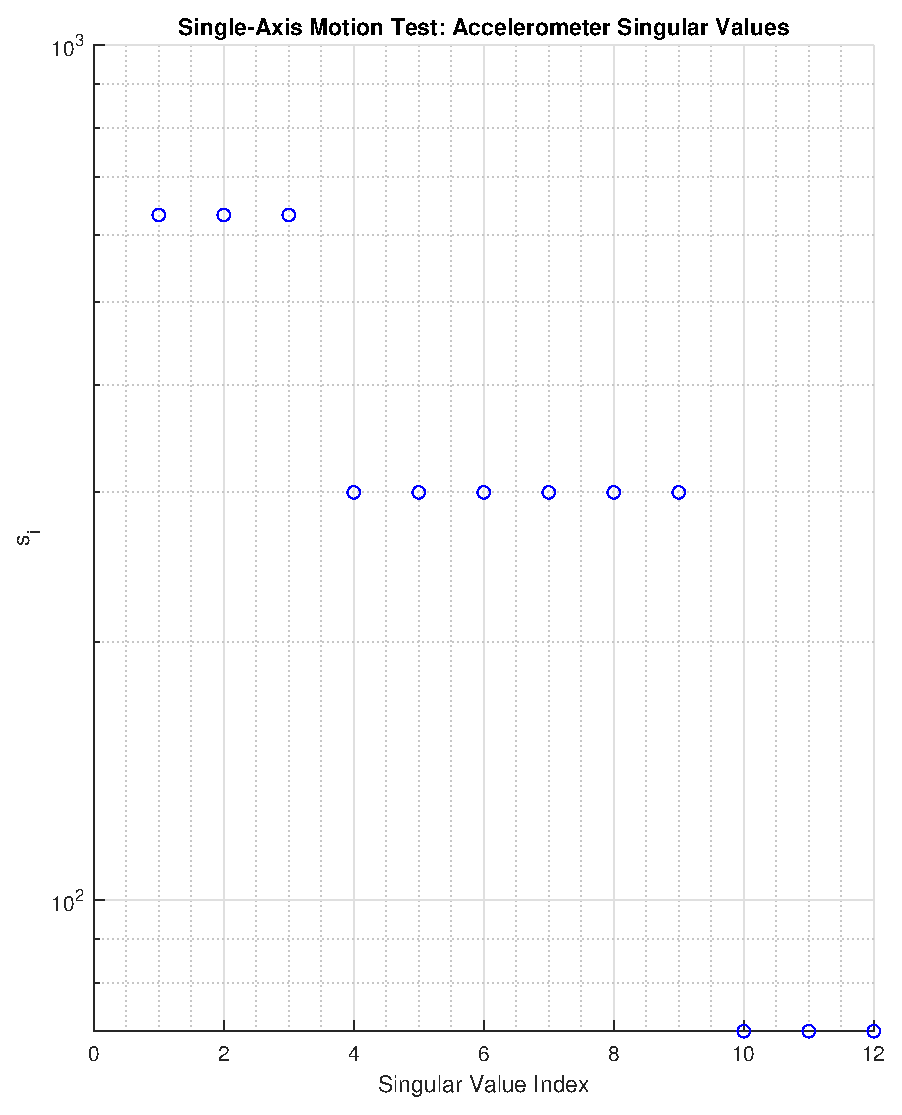
\includegraphics[width=0.65\textwidth]{./images/SAM_accel_singular_values.eps}
	\caption{Accelerometer Singular Values}
	\label{fig: single-axis accelerometer singular values}
\end{figure}
\FloatBarrier

\begin{figure}[h] 
	\centering
	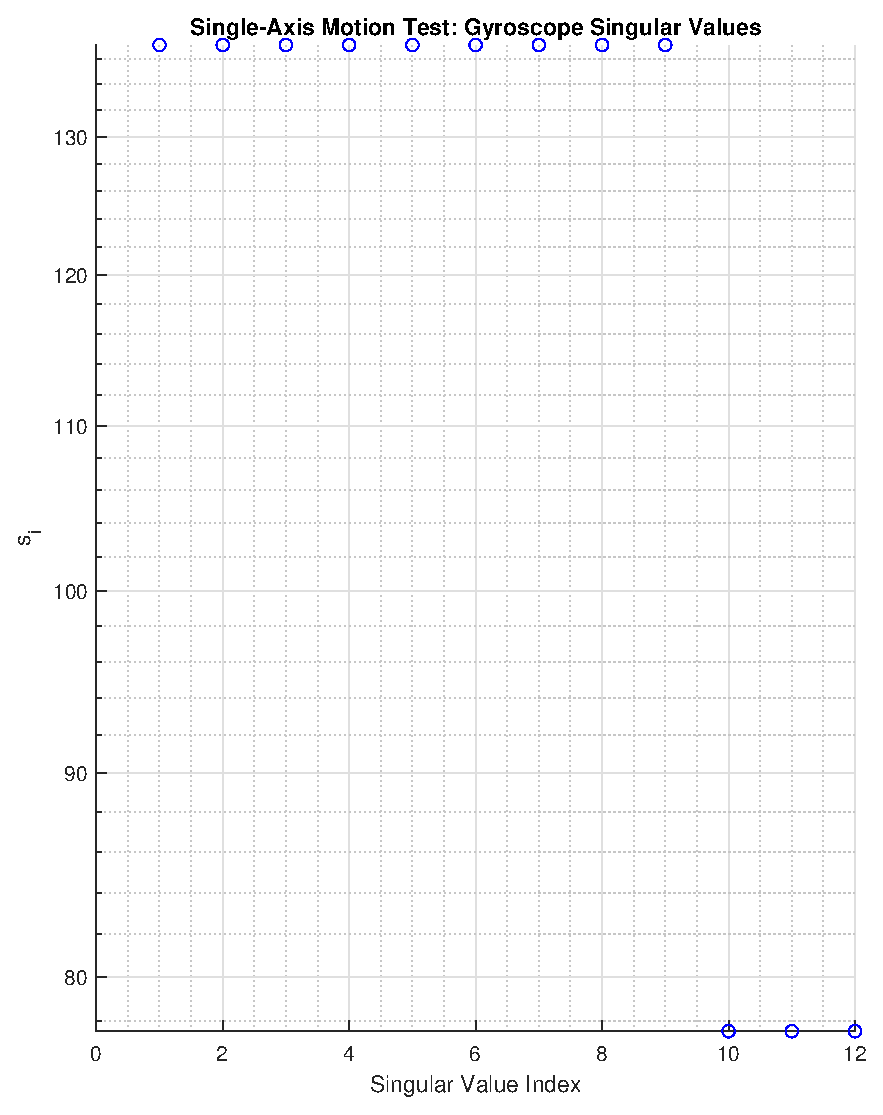
\includegraphics[width=0.65\textwidth]{./images/SAM_gyro_singular_values.eps}
	\caption{Gyroscope Singular Values}
	\label{fig: single-axis gyroscope singular values}
\end{figure}
\FloatBarrier


\subsubsection{Estimated Model Parameters}

The estimated model parameters and their associated errors are provided in figures \ref{fig: single-axis accelerometer parameters}, \ref{fig: single-axis accelerometer parameter error}, \ref{fig: single-axis gyroscope parameters}, and \ref{fig: single-axis gyroscope parameter error}. 

\begin{figure}[h] 
	\centering
	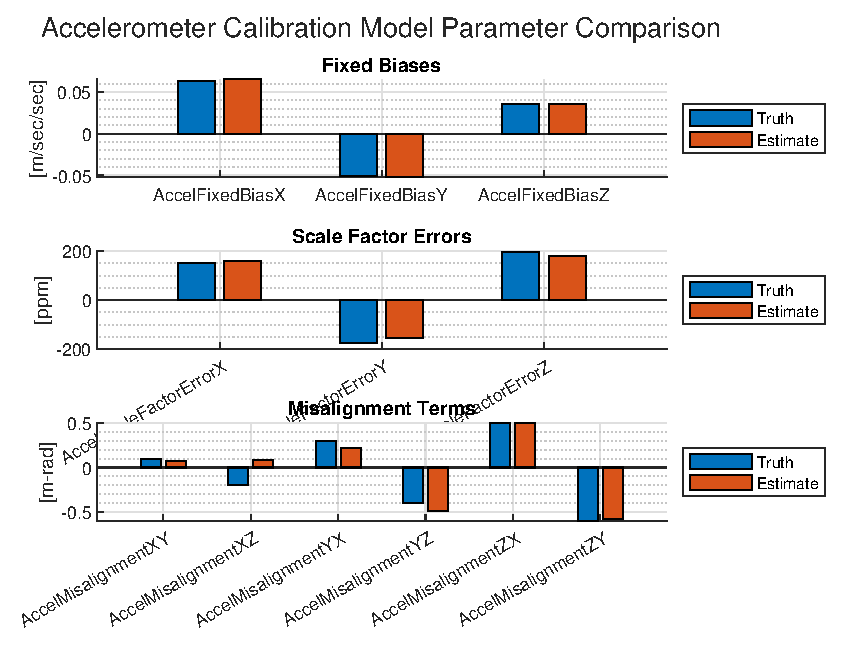
\includegraphics[width=0.65\textwidth]{./images/SAM_accel_model_parameters.eps}
	\caption{Estimated Accelerometer Model Parameters}
	\label{fig: single-axis accelerometer parameters}
\end{figure}
\FloatBarrier

\begin{figure}[h] 
	\centering
	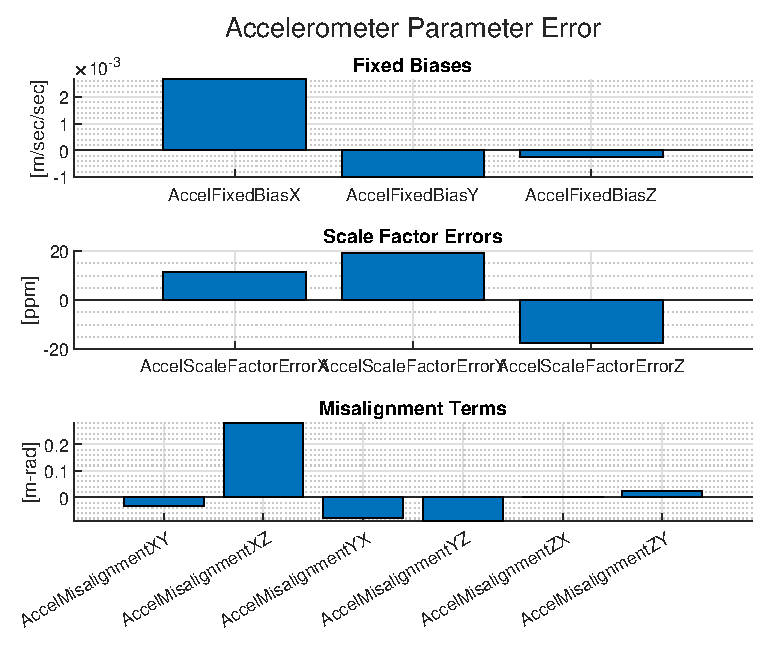
\includegraphics[width=0.65\textwidth]{./images/SAM_accel_model_error.eps}
	\caption{Accelerometer Model Parameter Error}
	\label{fig: single-axis accelerometer parameter error}
\end{figure}
\FloatBarrier

\begin{figure}[h] 
	\centering
	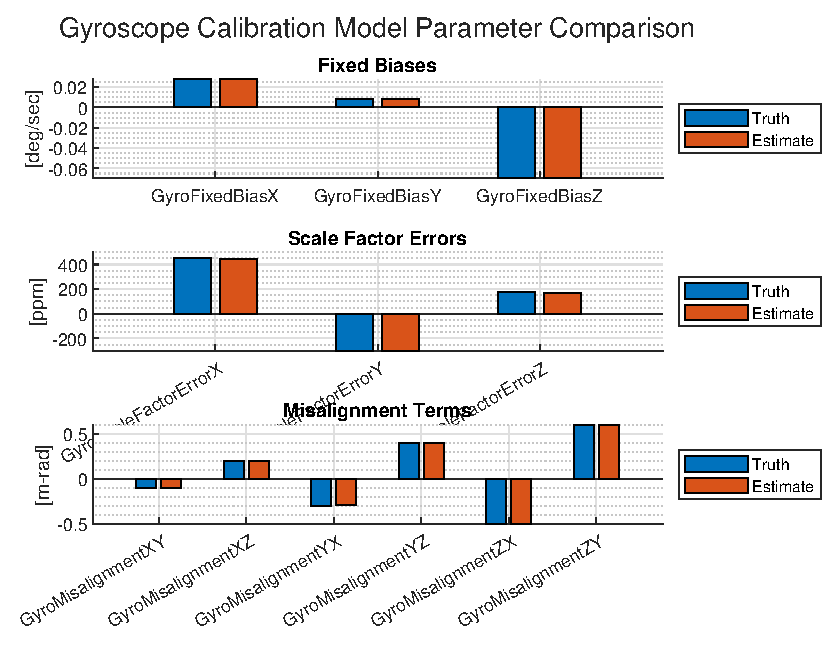
\includegraphics[width=0.65\textwidth]{./images/SAM_gyro_model_parameters.eps}
	\caption{Estimated Gyroscope Model Parameters}
	\label{fig: single-axis gyroscope parameters}
\end{figure}
\FloatBarrier

\begin{figure}[h] 
	\centering
	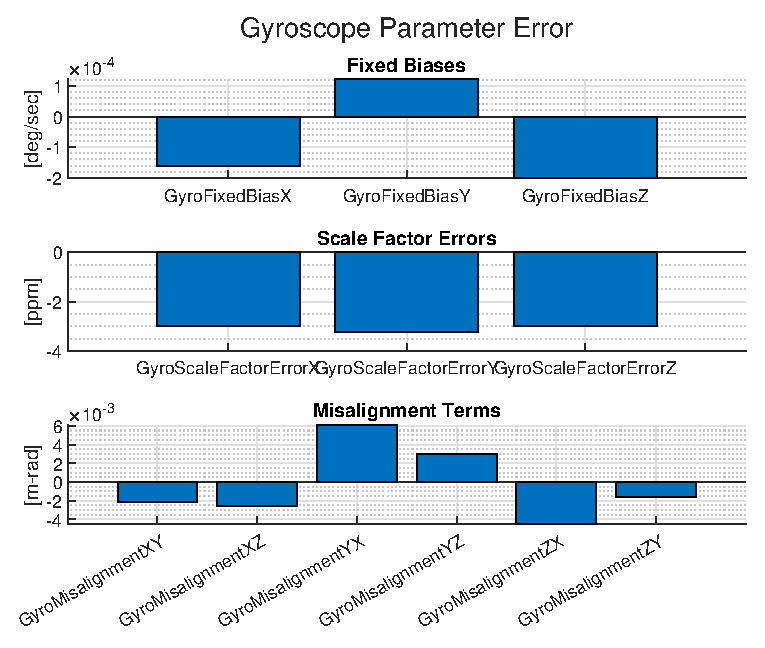
\includegraphics[width=0.65\textwidth]{./images/SAM_gyro_model_error.eps}
	\caption{Gyroscope Model Parameter Error}
	\label{fig: single-axis gyroscope parameter error}
\end{figure}
\FloatBarrier


\subsubsection{Model Covariance and 95\% Confidence Bounds}

In preparation for formulating a weighted least squares solution, the weighted matrices were used to compute the model covariance and resulting 95\% confidence bounds. 

\begin{figure}[h] 
	\centering
	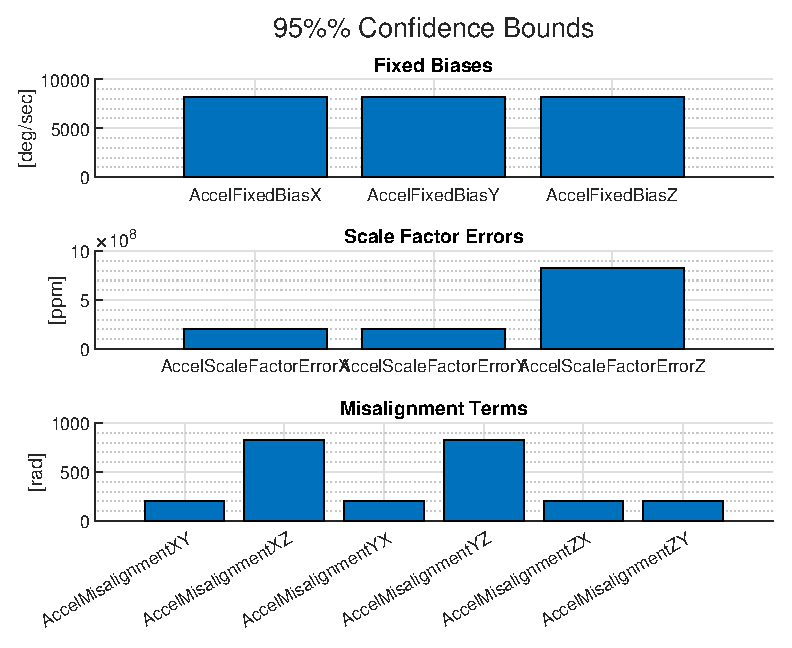
\includegraphics[width=0.65\textwidth]{./images/SAM_accel_model_95_confidence_bounds.eps}
	\caption{Accelerometer 95\% Confidence Bounds}
	\label{fig: single-axis accel 95 confidence bounds}
\end{figure}
\FloatBarrier

\begin{figure}[h] 
	\centering
	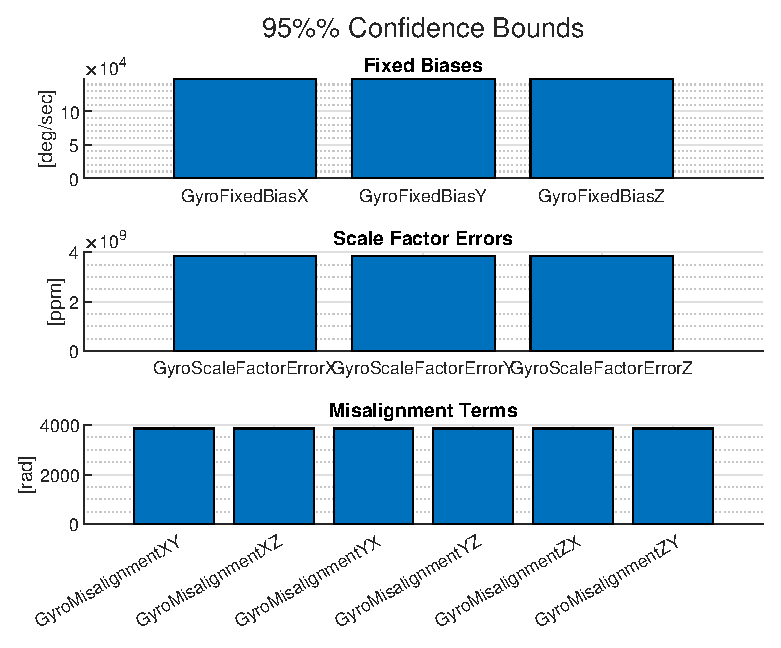
\includegraphics[width=0.65\textwidth]{./images/SAM_gyro_model_95_confidence_bounds.eps}
	\caption{Gyroscope 95\% Confidence Bounds}
	\label{fig: single-axis gyro 95 confidence bounds}
\end{figure}
\FloatBarrier

In each case, the confidence bounds are wildly higher than the error actually achieved through the generalized model inverse solution!
















%******************************************************
% Multi-Axis Motion
%******************************************************

\subsection{Multi-Axis Motion Calibration Sequence}

In response to still lacking full rank with the single-axis motion calibration sequences, yet another calibration sequence was designed to put axis of the UUT in motion at the same time in hopes of establishing model operators of full rank. Figures \ref{fig: multi-axis angular velocity profile} and \ref{fig: multi-axis euler angle profile} show the designed motion profile.

\begin{figure}[h] 
	\centering
	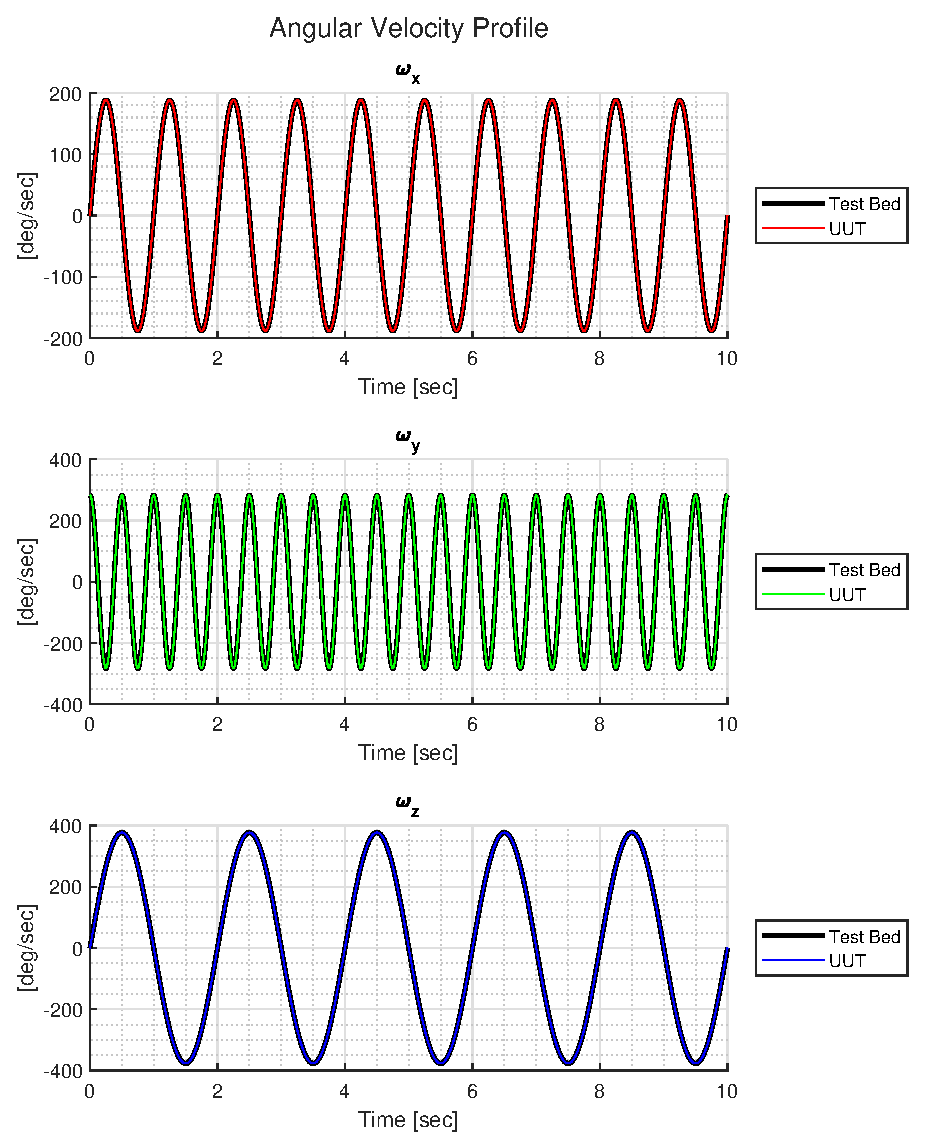
\includegraphics[width=0.65\textwidth]{./images/MAM_angular_velocity_profile.eps}
	\caption{Multi-Axis Angular Velocity Profile}
	\label{fig: multi-axis angular velocity profile}
\end{figure}
\FloatBarrier

\begin{figure}[h] 
	\centering
	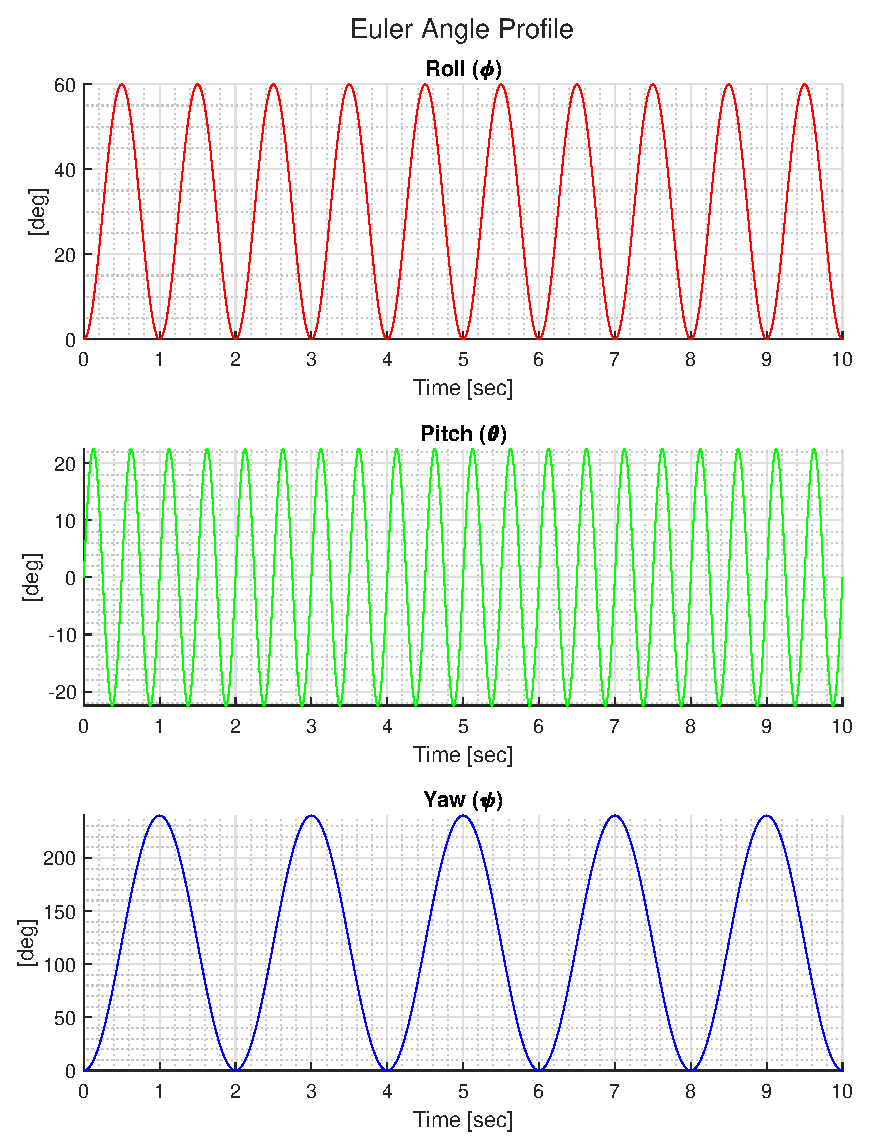
\includegraphics[width=0.65\textwidth]{./images/MAM_euler_angle_profile.eps}
	\caption{Multi-Axis Euler Angle Profile}
	\label{fig: multi-axis euler angle profile}
\end{figure}
\FloatBarrier

Due to the rotations of the test bed, the specific force is also altered as shown in figure \ref{fig: multi-axis specific force profile}.

\begin{figure}[h] 
	\centering
	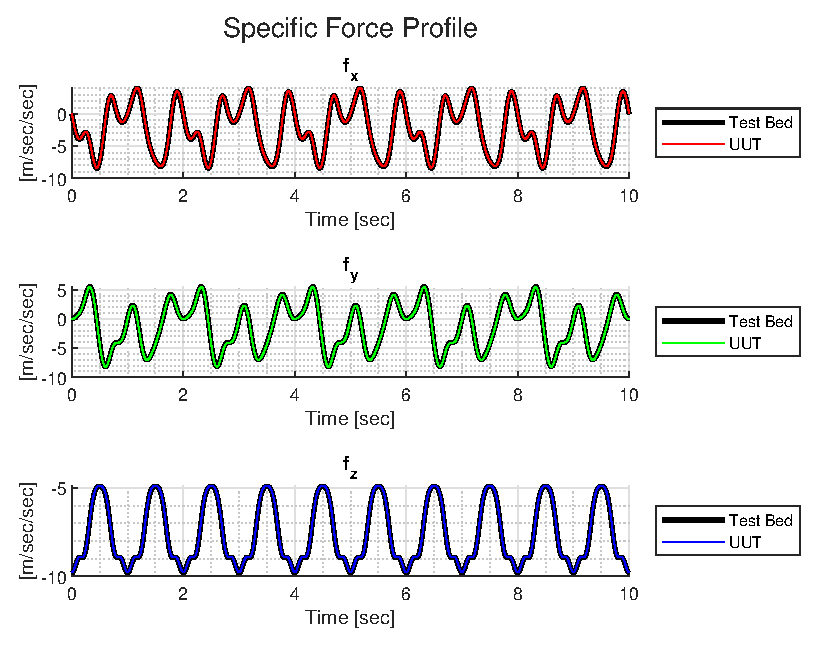
\includegraphics[width=0.65\textwidth]{./images/MAM_specific_force_profile.eps}
	\caption{Multi-Axis Specific Force Profile}
	\label{fig: multi-axis specific force profile}
\end{figure}
\FloatBarrier

\subsubsection{Model Operator Rank}

Even with new motion profiles, both model operators $G_a$ and $G_g$ are not full rank. 

\begin{align}
	\textrm{rank}\left(G_a\right) &= 12,\,\,\, G_a \in \R^{909 \times 12} \notag\\
	\\
	\textrm{rank}\left(G_g\right) &= 12,\,\,\, G_g \in \R^{909 \times 12} \notag
\end{align}

In response, a model solution was still obtained using the generalized inverse. This rank-deficiency is of the type "$p = n$ and $p < m$, in which the data null space is non-trivial but the model null space is trivial. This implies that the solution will be unique, but cannot fit the general data exactly. For both $G_a$ and $G_g$, a singular value decomposition (SVD) was performed and each decomposed matrix was truncated to the rank of the matrix. The generalized inverse model was formed accordingly below.

\begin{align}
	\bv{m}_{\dagger}^{a} &= V_{a,p} S_{a,p}^{-1} U_{a,p}^T \bv{d}_a \notag\\
	\\
	\bv{m}_{\dagger}^{g} &= V_{g,p} S_{g,p}^{-1} U_{g,p}^T \bv{d}_g \notag
\end{align}

Each model resolution matrix $R_m = V_p V_p^T$ shows that each model parameter has perfect resolution. The singular values for each model operator are shown in figures \ref{fig: multi-axis accelerometer singular values} and \ref{fig: multi-axis gyroscope singular values}. 

\begin{figure}[h] 
	\centering
	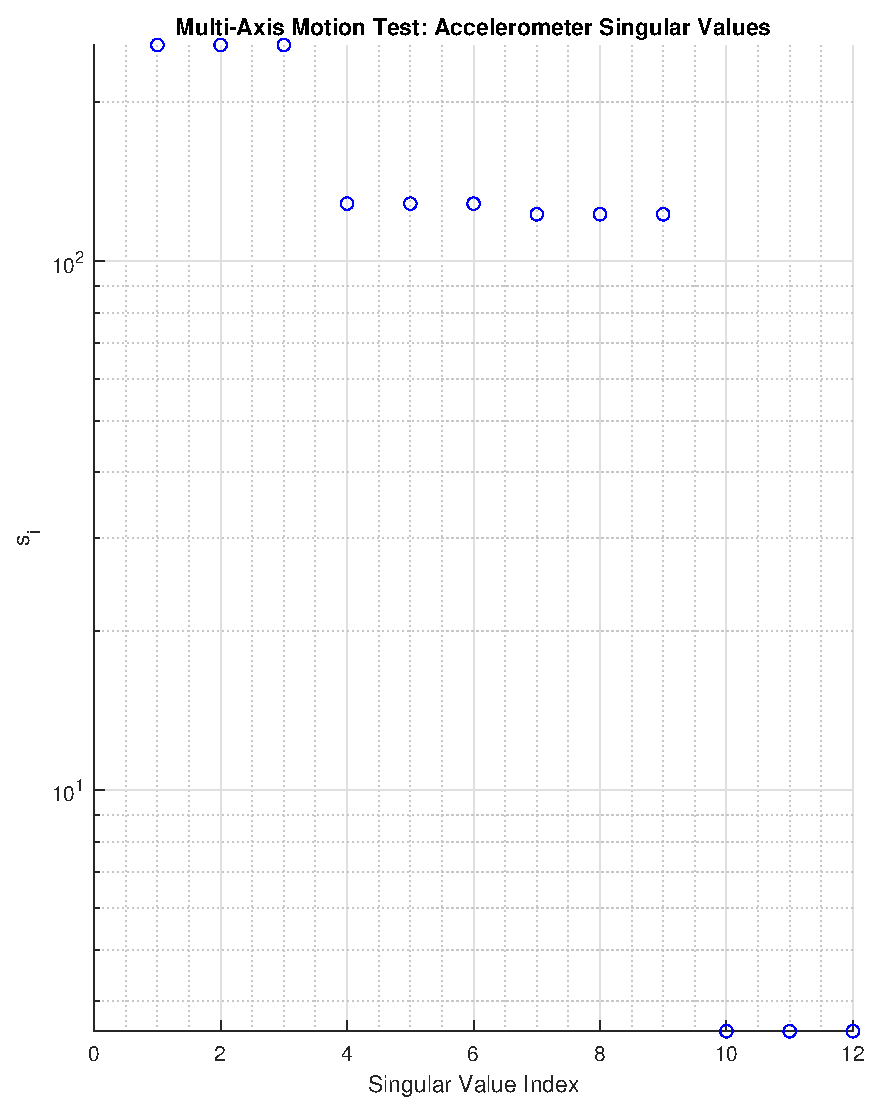
\includegraphics[width=0.65\textwidth]{./images/MAM_accel_singular_values.eps}
	\caption{Accelerometer Singular Values}
	\label{fig: multi-axis accelerometer singular values}
\end{figure}
\FloatBarrier

\begin{figure}[h] 
	\centering
	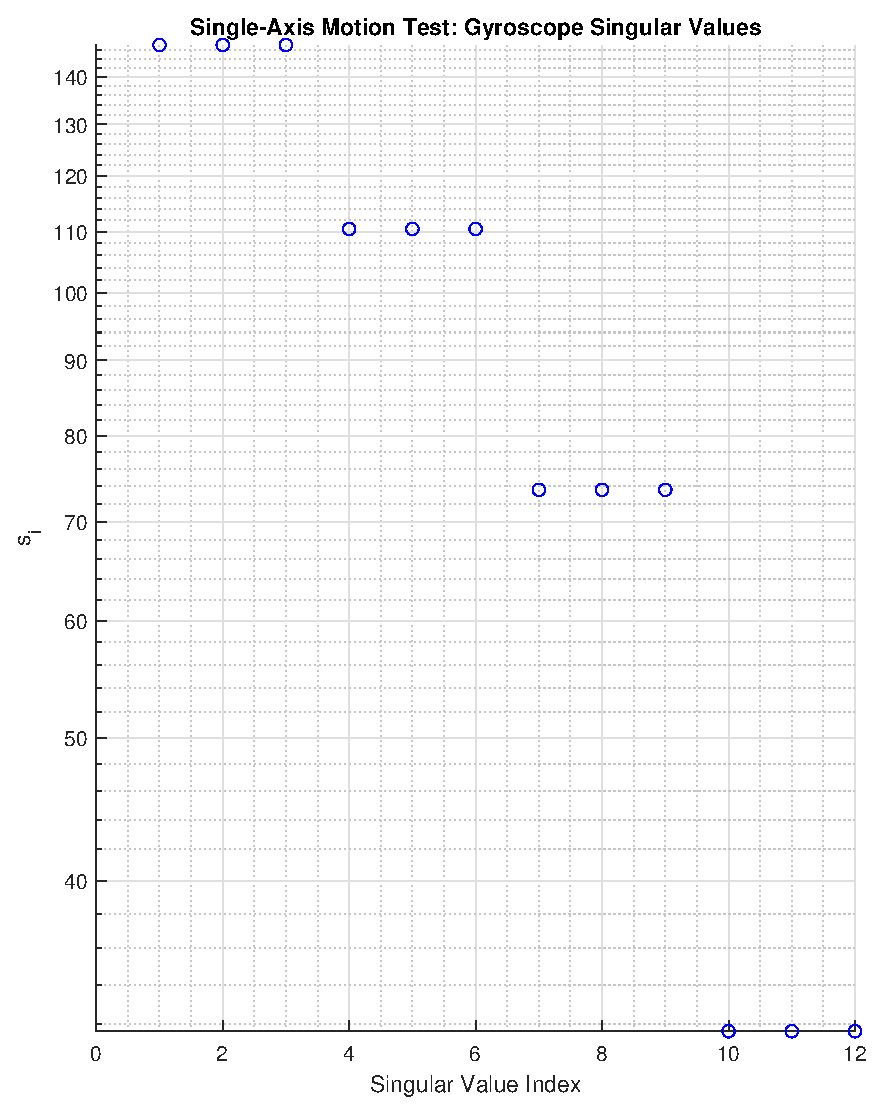
\includegraphics[width=0.65\textwidth]{./images/MAM_gyro_singular_values.eps}
	\caption{Gyroscope Singular Values}
	\label{fig: multi-axis gyroscope singular values}
\end{figure}
\FloatBarrier


\subsubsection{Estimated Model Parameters}

The estimated model parameters and their associated errors are provided in figures \ref{fig: multi-axis accelerometer parameters}, \ref{fig: multi-axis accelerometer parameter error}, \ref{fig: multi-axis gyroscope parameters}, and \ref{fig: multi-axis gyroscope parameter error}. 

\begin{figure}[h] 
	\centering
	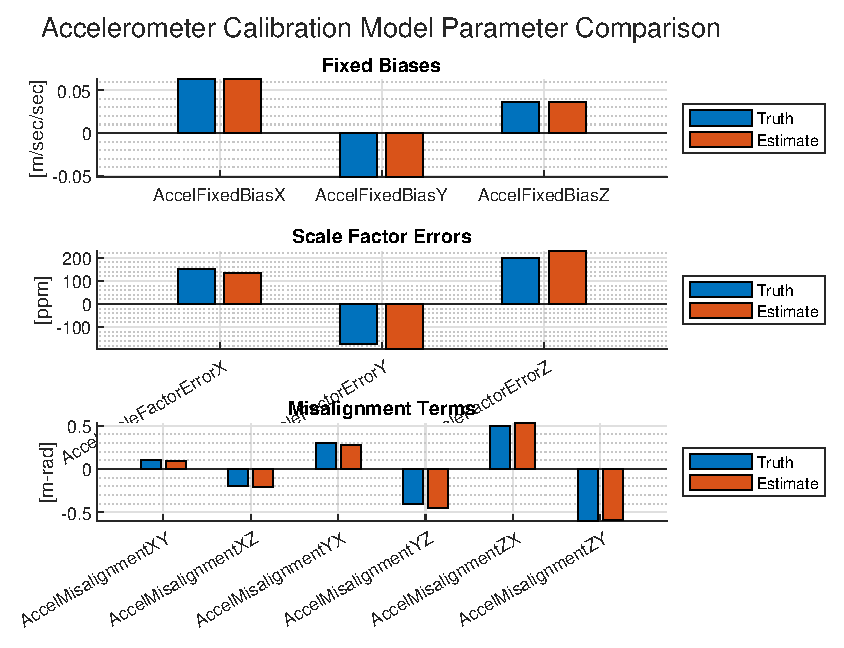
\includegraphics[width=0.65\textwidth]{./images/MAM_accel_model_parameters.eps}
	\caption{Estimated Accelerometer Model Parameters}
	\label{fig: multi-axis accelerometer parameters}
\end{figure}
\FloatBarrier

\begin{figure}[h] 
	\centering
	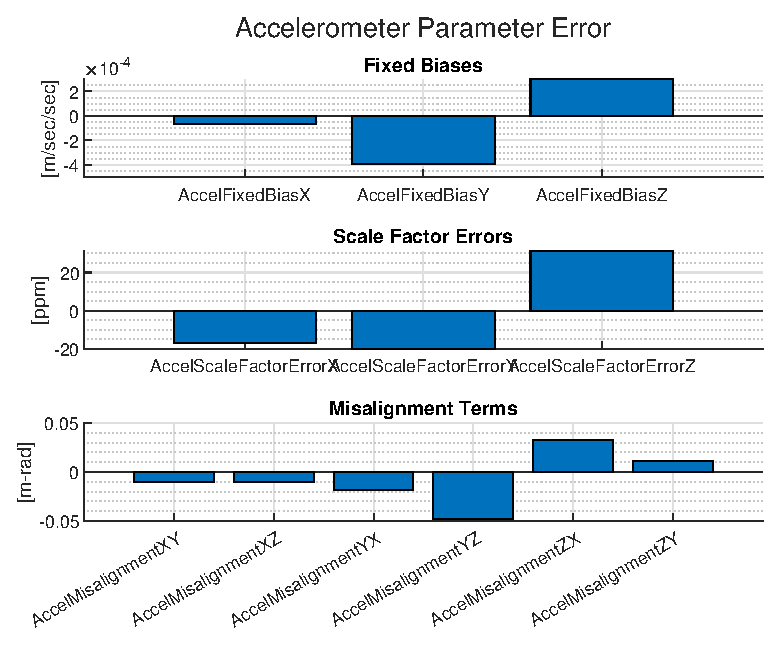
\includegraphics[width=0.65\textwidth]{./images/MAM_accel_model_error.eps}
	\caption{Accelerometer Model Parameter Error}
	\label{fig: multi-axis accelerometer parameter error}
\end{figure}
\FloatBarrier

\begin{figure}[h] 
	\centering
	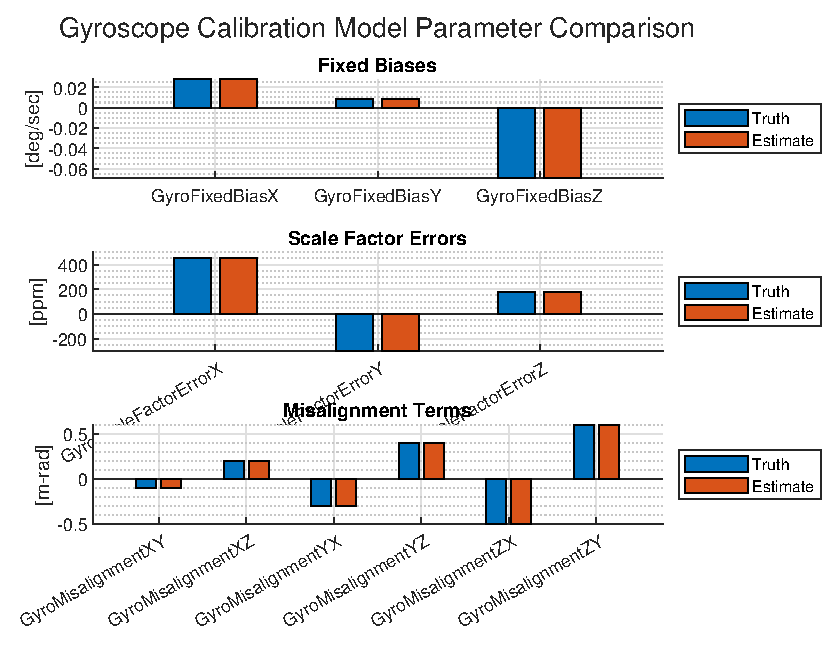
\includegraphics[width=0.65\textwidth]{./images/MAM_gyro_model_parameters.eps}
	\caption{Estimated Gyroscope Model Parameters}
	\label{fig: multi-axis gyroscope parameters}
\end{figure}
\FloatBarrier

\begin{figure}[h] 
	\centering
	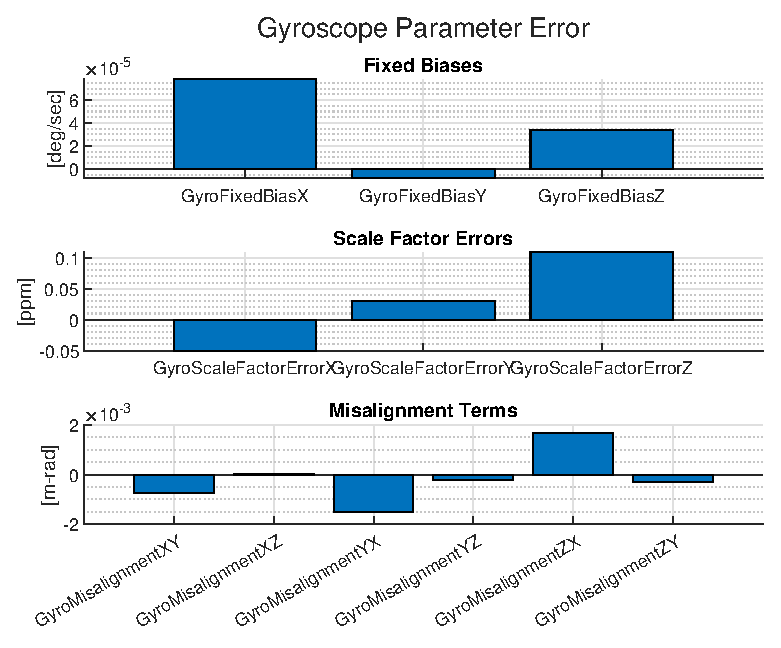
\includegraphics[width=0.65\textwidth]{./images/MAM_gyro_model_error.eps}
	\caption{Gyroscope Model Parameter Error}
	\label{fig: multi-axis gyroscope parameter error}
\end{figure}
\FloatBarrier


\subsubsection{Model Covariance and 95\% Confidence Bounds}

In preparation for formulating a weighted least squares solution, the weighted matrices were used to compute the model covariance and resulting 95\% confidence bounds. 

\begin{figure}[h] 
	\centering
	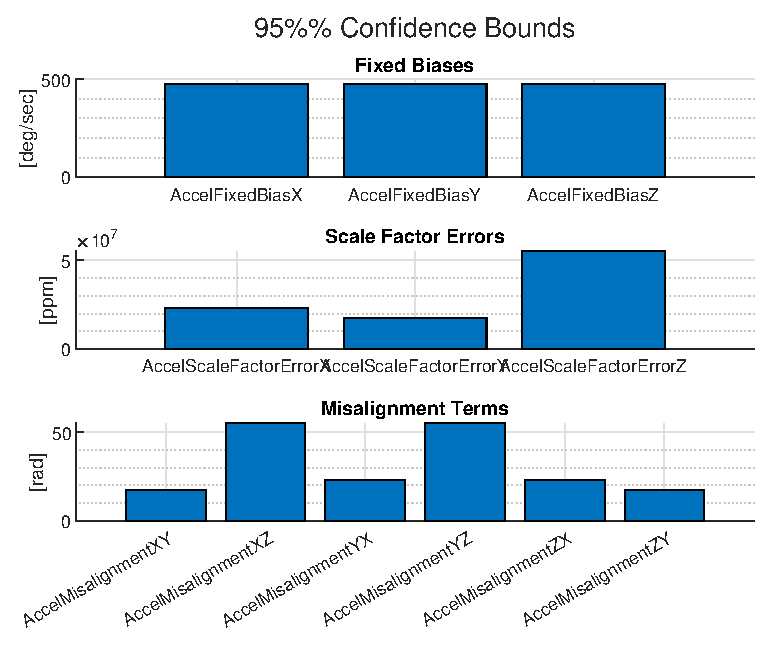
\includegraphics[width=0.65\textwidth]{./images/MAM_accel_model_95_confidence_bounds.eps}
	\caption{Accelerometer 95\% Confidence Bounds}
	\label{fig: multi-axis accel 95 confidence bounds}
\end{figure}
\FloatBarrier

\begin{figure}[h] 
	\centering
	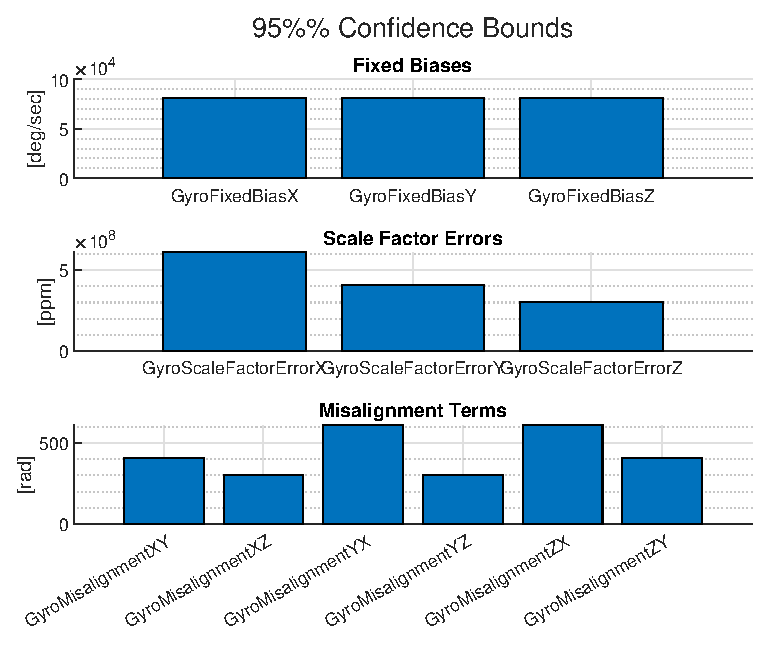
\includegraphics[width=0.65\textwidth]{./images/MAM_gyro_model_95_confidence_bounds.eps}
	\caption{Gyroscope 95\% Confidence Bounds}
	\label{fig: multi-axis gyro 95 confidence bounds}
\end{figure}
\FloatBarrier

In each case, the confidence bounds are wildly higher than the error actually achieved through the generalized model inverse solution!



	
	\newpage
	%----------------------------------------------------------------------
% Discussion

\begingroup
\allowdisplaybreaks

\section{Discussion}

\subsection{A Comparison to the Traditional Means of Calibration}

It was unexpected that the model operators built from the traditional calibration data sets to be rank-deficient, blocking the opportunity to make a meaningful comparison. However, this obstacle is still impactful to the navigation community for those that have large amounts of legacy calibration data. This result implies that those that wish to upgrade to a systematic means of IMU calibration must collect new data with new motion profiles! The traditional methods for IMU calibration are not sufficient for systematic calibration.

\subsection{A Comparison of the Three Motion Profiles}

When designing new motion profiles to upgrade to systematic calibration, careful consideration is required to determine how the singular values, model errors, model covariances, and model parameter correlation are impacted. This comparison covers three different motion profiles. Each fitted model from the three motion profiles are compared in figure \ref{fig: parameter comparsion}.

\begin{figure}[!h] 
	\centering
	\includegraphics[width=0.49\textwidth]{./images/gyro_parameter_comparison.eps} \hfill
	\includegraphics[width=0.49\textwidth]{./images/accel_parameter_comparison.eps}
	\caption{Calibration Parameter Comparison}
	\label{fig: parameter comparsion}
\end{figure}
\FloatBarrier

Note that the least squares solution for each motion profile is relatively close to the true model parameters. In each case, there are no extreme outliers that indicate any large error. Similarly, figure \ref{fig: parameter error comparsion} provides the error of each model parameter for each motion profile. 

\begin{figure}[!h] 
	\centering
	\includegraphics[width=0.49\textwidth]{./images/gyro_parameter_error_comparison.eps} \hfill
	\includegraphics[width=0.49\textwidth]{./images/accel_parameter_error_comparison.eps}
	\caption{Calibration Parameter Error Comparison}
	\label{fig: parameter error comparsion}
\end{figure}
\FloatBarrier

In almost all cases, the second motion profile seems to yield the least amount of model error, while the first motion profile yields the most error. In a few cases the third motion profile outperforms the second motion profile, but it is surprising the third motion profile did not perform equally well. The model covariances and resulting confidence intervals follow a similar trend, shown in figures \ref{fig: parameter covariance comparsion} and \ref{fig: parameter conf95 comparsion}. 

\begin{figure}[!h] 
	\centering
	\includegraphics[width=0.49\textwidth]{./images/gyro_parameter_covariance_comparison.eps} \hfill
	\includegraphics[width=0.49\textwidth]{./images/accel_parameter_covariance_comparison.eps}
	\caption{Calibration Parameter Covariance Comparison}
	\label{fig: parameter covariance comparsion}
\end{figure}
\FloatBarrier

\begin{figure}[!h] 
	\centering
	\includegraphics[width=0.49\textwidth]{./images/gyro_parameter_conf95_comparison.eps} \hfill
	\includegraphics[width=0.49\textwidth]{./images/accel_parameter_conf95_comparison.eps}
	\caption{Calibration Parameter Confidence Interval Comparison}
	\label{fig: parameter conf95 comparsion}
\end{figure}
\FloatBarrier

Notice that the covariances associated with the gyroscope scale factor and misalignment parameters are incredibly high, which is likely due to the correlation among these parameters shown in figure \ref{fig: MP3 correlation matrix}. This might also explain why the second motion profile yielded much better performance for the accelerometer parameters, which is when the least amount of parameter correlation was present as shown in figure \ref{fig: MP2 correlation matrix}. It seems that designing a motion profile that minimizes model parameter correlation is key to reducing the uncertainty for each calibration parameter. This insight is key for anyone calibrating IMUs for use in safety-critical systems where requirements may be stringent.

\subsection{IMU Calibration for Ill-Conditioned System Dynamics}





	
	\newpage
	%----------------------------------------------------------------------
% Conclusion

\begingroup
\allowdisplaybreaks

\section{Conclusion}

Inertial sensor calibration is an essential activity before installing an IMU into a self-driving vehicle for the purposes of navigation. Traditional calibration methods use simple tests on their respective rotational test beds and post-process the collected data in piece-meal sections to compute only the most basic of IMU error sources. In an effort to improve the status-quo, systematic calibration seeks to leverage batched estimation methods to extend model complexity and make use of all available information to estimate its model parameters. In addition, systematic calibration also establishes some measure of uncertainty for each model parameter which is useful for verifying the final calibration parameters used before vehicle application. 

Systematic calibration through the lens of inverse problem techniques provides opportunities to assess the conditioning of the discrete linear inverse problems formed. When comparing the same basic models used in traditional IMU calibration, unexpected difficulty in achieving a full-rank model operator required the use of forming generalized inverse solutions. Also model resolution was preserved in the formation of the solutions, there still remains unanswered questions about the covariance that can be assigned to each model parameter. In the end, the generalized model solutions were still surprisingly close to the true model parameters used in simulation. As a result, the resulting model parameters from the generalized inverse solution are still within an "adaquete" range for low-stakes navigation such as a hobbyist UAV. 
	
	%------------------------------------------------------------------
	% Print Bibliography
	
	\newpage
	\bibliographystyle{ieeetr}
	\bibliography{references}
	
	%------------------------------------------------------------------
	% Print Appendix
	
	\newpage
	%----------------------------------------------------------------------
% Appedix

\begingroup
\allowdisplaybreaks

\section{Appendix}

\subsection{Traditional IMU Calibration Post-Processing} \label{sec: traditional imu calibration post-processing}

From equation \ref{eq: expanded IMU forward error model} and collected test data listed in table \ref{tab: traditional_calibration_tests}, the accelerometer bias $\bv{b}_a$ can be solved from the collected test data.

\begin{align} \label{eq: traditional accel bias computation}
	\bv{b}_a = \begin{bmatrix} b_{a,x} \\ \\ b_{a,y} \\ \\ b_{a,z} \end{bmatrix} = \frac{1}{2} \begin{bmatrix}
		\bar{f}^{\,+\textrm{x}}_{x} + \bar{f}^{\,-\textrm{x}}_{x} \\
		\\
		\bar{f}^{\,+\textrm{y}}_{y} + \bar{f}^{\,-\textrm{y}}_{y} \\
		\\
		\bar{f}^{\,+\textrm{z}}_{z} + \bar{f}^{\,-\textrm{z}}_{z}
	\end{bmatrix}
\end{align}

Likewise, accelerometer scale factor terms within the quantity $M_a$ can also be computed, where $g$ is the magnitude of the accelerometer due to gravity at that specific location at the inertial test laboratory.

\begin{align} \label{eq: traditional accel scale factor computation}
	\bv{s}_a = \begin{bmatrix} s_{a,x} \\ \\ s_{a,y} \\ \\ s_{a,z} \end{bmatrix} = \frac{1}{2g} \begin{bmatrix}
		\bar{f}^{\,+\textrm{x}}_{x} - \bar{f}^{\,-\textrm{x}}_{x} \\
		\\
		\bar{f}^{\,+\textrm{y}}_{y} - \bar{f}^{\,-\textrm{y}}_{y} \\
		\\
		\bar{f}^{\,+\textrm{z}}_{z} - \bar{f}^{\,-\textrm{z}}_{z}
	\end{bmatrix} - 1
\end{align}

Accelerometer misalignment uses off-axis terms from each collected test where each misalignment term is computed separately.

\begin{align} \label{eq: traditional accel misalignment computation}
	m_{a,xy} &= \frac{1}{2g} \left( \bar{f}^{\,+\textrm{y}}_{x} - \bar{f}^{\,-\textrm{y}}_{x} \right) \notag\\
	\notag\\
	m_{a,xz} &= \frac{1}{2g} \left( \bar{f}^{\,+\textrm{z}}_{x} - \bar{f}^{\,-\textrm{z}}_{x} \right) \notag\\
	\notag\\
	m_{a,yx} &= \frac{1}{2g} \left( \bar{f}^{\,+\textrm{x}}_{y} - \bar{f}^{\,-\textrm{x}}_{y} \right) \notag\\
	\\
	m_{a,yz} &= \frac{1}{2g} \left( \bar{f}^{\,+\textrm{z}}_{y} - \bar{f}^{\,-\textrm{z}}_{y} \right) \notag\\
	\notag\\
	m_{a,zx} &= \frac{1}{2g} \left( \bar{f}^{\,+\textrm{x}}_{z} - \bar{f}^{\,-\textrm{x}}_{z} \right) \notag\\
	\notag\\
	m_{a,zy} &= \frac{1}{2g} \left( \bar{f}^{\,+\textrm{y}}_{z} - \bar{f}^{\,-\textrm{y}}_{z} \right) \notag
\end{align}

Also from equation \ref{eq: expanded IMU forward error model}, the gyroscope bias $\bv{b}_g$ can be solved from the collected test data.

\begin{align} \label{eq: traditional gyro bias computation}
	\bv{b}_g = \begin{bmatrix} b_{a,x} \\ \\ b_{a,y} \\ \\ b_{a,z} \end{bmatrix} = \frac{1}{2} \begin{bmatrix}
		\bar{\omega}^{\,+\textrm{x}}_{x} + \bar{\omega}^{\,-\textrm{x}}_{x} \\
		\\
		\bar{\omega}^{\,+\textrm{y}}_{y} + \bar{\omega}^{\,-\textrm{y}}_{y} \\
		\\
		\bar{\omega}^{\,+\textrm{z}}_{z} + \bar{\omega}^{\,-\textrm{z}}_{z}
	\end{bmatrix}
\end{align}

Gyroscope scale factor terms within the quantity $M_g$ can also be computed, where $\omega_{\textrm{test}}$ is the magnitude of the accelerometer due to gravity at that specific location at the inertial test laboratory.

\begin{align} \label{eq: traditional gyro scale factor computation}
	\bv{s}_g = \begin{bmatrix} s_{g,x} \\ \\ s_{g,y} \\ \\ s_{g,z} \end{bmatrix} = \frac{1}{2\omega_{\textrm{test}}} \begin{bmatrix}
		\bar{\omega}^{\,+\textrm{x}}_{x} - \bar{\omega}^{\,-\textrm{x}}_{x} \\
		\\
		\bar{\omega}^{\,+\textrm{y}}_{y} - \bar{\omega}^{\,-\textrm{y}}_{y} \\
		\\
		\bar{\omega}^{\,+\textrm{z}}_{z} - \bar{\omega}^{\,-\textrm{z}}_{z}
	\end{bmatrix} - 1
\end{align}

Gyroscope misalignment uses off-axis terms from each collected test where each misalignment term is computed separately.

\begin{align} \label{eq: traditional gyro misalignment computation}
	m_{g,xy} &= \frac{1}{2\omega_{\textrm{test}}} \left( \bar{\omega}^{\,+\textrm{y}}_{x} - \bar{\omega}^{\,-\textrm{y}}_{x} \right) \notag\\
	\notag\\
	m_{g,xz} &= \frac{1}{2\omega_{\textrm{test}}} \left( \bar{\omega}^{\,+\textrm{z}}_{x} - \bar{\omega}^{\,-\textrm{z}}_{x} \right) \notag\\
	\notag\\
	m_{g,yx} &= \frac{1}{2\omega_{\textrm{test}}} \left( \bar{\omega}^{\,+\textrm{x}}_{y} - \bar{\omega}^{\,-\textrm{x}}_{y} \right) \notag\\
	\\
	m_{g,yz} &= \frac{1}{2\omega_{\textrm{test}}} \left( \bar{\omega}^{\,+\textrm{z}}_{y} - \bar{\omega}^{\,-\textrm{z}}_{y} \right) \notag\\
	\notag\\
	m_{g,zx} &= \frac{1}{2\omega_{\textrm{test}}} \left( \bar{\omega}^{\,+\textrm{x}}_{z} - \bar{\omega}^{\,-\textrm{x}}_{z} \right) \notag\\
	\notag\\
	m_{g,zy} &= \frac{1}{2\omega_{\textrm{test}}} \left( \bar{\omega}^{\,+\textrm{y}}_{z} - \bar{\omega}^{\,-\textrm{y}}_{z} \right) \notag
\end{align}
	
	
\end{document}


%----------------------------------------------------------------------
% Additional Copy-and-Paste Templates

% Figure

%\begin{figure}[h] \label{fig: my figure}
%	\centering
%	\includegraphics[width=0.8\textwidth]{./images/<image.png>}
%	\caption{\textcolor{red}{provide a caption}}
%\end{figure}


% Table

%\begin{center}
%	\begin{tabular} { | h1 | h2 | h3 | } \label{tab: my table}
	%		
	%		\hline
	%		x11 & x12 & x13 \\
	%		\hline
	%		x21 & x22 & x23 \\
	%		\hline
	%		x31 & x32 & x33 \\
	%		\hline
	%		
	%	\end{tabular}
%	\caption{\textcolor{red}{put caption here}
	%\end{center}
